\documentclass[10pt]{article}
\newcommand\tab[1][1cm]{\hspace*{#1}}
\usepackage{amsmath}
\usepackage{graphicx}
\newcommand{\ihat}{\boldsymbol{\hat{\textbf{\i}}}}
\newcommand{\jhat}{\boldsymbol{\hat{\textbf{\j}}}}
\graphicspath{ {./} }
\usepackage[margin=1in]{geometry}
\begin{document}

\paragraph{Nicole Pagane $|$ 05/02/19 }

\section*{Final Project Progress: Transcriptional Chromatin Dynamics}

\subsection*{Physical Problem}
I am interested in characterizing a potential mechanism for nucleosome dynamics under transcription. Essentially, DNA is very compact (of which the basis packaging unit is called a nucleosome) and needs to allow for transcription to make proteins. The process of transcription requires a bulky protein (called RNA polymerase II or RNAP) shuttling along the DNA---and thus the progression of RNAP would seemingly be interrupted by bulky/compact nucleosomes distributed along the gene). Though complete eviction of nucleosomes from the gene would seem a reasonable prerequisite for transcription, this is not the case. It has been shown that after a round of transcription---i.e. one passage of RNAP along the gene---the nucleosomes shift in the opposite direction of RNAP progression (Kulaeva et al. 2014). While this mechanism is not entirely understood, it has been conjectured to be mediated through the looping of unwound DNA in front of RNAP to allow for the transfer of the nucleosome upstream to avoid RNAP. I am interested in characterizing this process through modeling DNA as a worm-like chain to explore the energy penalty of loop formation, where the energy required to bend a polymer can be described through:
\begin{equation}
E = \frac{1}{2}k_BT\int_0^{L_0}P\cdot(\frac{\delta^2\vec{r}(s)}{\delta s^2})^2ds
\end{equation}
where $T$ is the temperature, $L_0$ is the maximum length of the straightened polymer, $P$ is the characteristic persistence length of the polymer, and $\vec{r}(2)$ is the parametrized path of the polymer where $s \in (0, L_0)$. The persistence length $P$ of DNA is between 40-50 nm.
\subsection*{Numerical Solution}
 I have constructed a two-dimensional curve to represent the potential looping mechanism of this transcriptional process, visualized below with orange representing RNAP, blue representing a nucleosome comprised of 8 protein subunits (the preferred state), and the red representing a nucleosome comprised of 6 protein subunits (the less stable state). The looping would allow for the nucleosomes to move upstream and avoid collision with RNAP. Some model constraints to consider is the forced 90 degree bend of DNA inflicted by RNAP for transcription, the total length of the DNA needed for this transfer process, and the distance required for successful nucleosome transfer upstream.
  \begin{figure}[!htb]
    \begin{minipage}{\textwidth}
     \caption{Looping DNA with Nucleosomes}
     \centering
     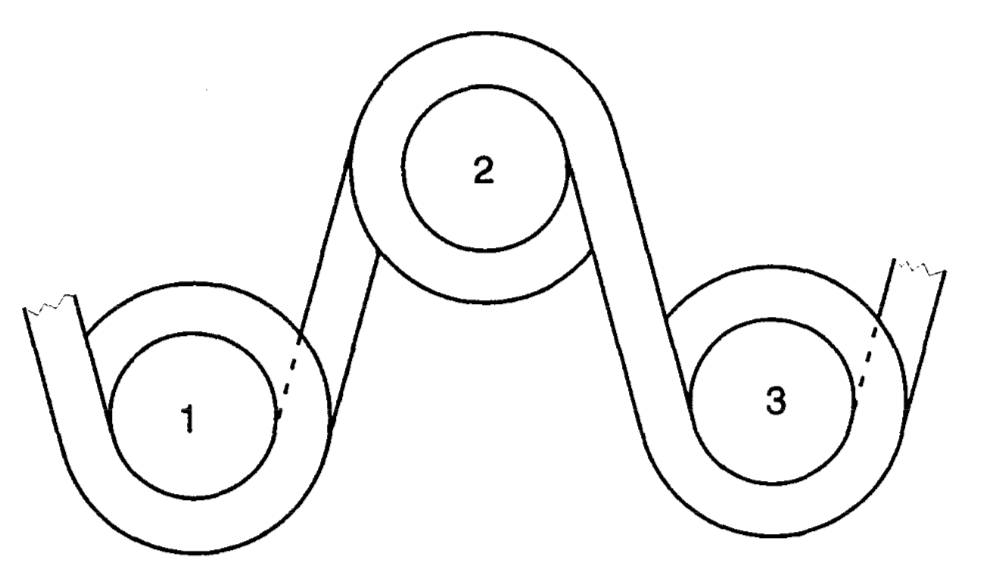
\includegraphics[width=0.6\textwidth]{hi.png}
   \end{minipage}\hfill
 \end{figure}\\
  The general formula to create these two-dimensional DNA loops were as follows:
 \begin{equation}
 l(x) = cr\sin{\frac{x}{r}} + \frac{1}{x} - sr
 \end{equation}
where $c$ allows for scaling of the loop, $\frac{1}{x}$ allows for the near 90 degree bend introduced by RNAP, and $s$ is modulated to optimize the transfer distance. While I am modulating these parameters to fit this equation to literature values, I may want to try and construct some system of linear equations to solve for the best parameter set rather than through trial-and-error. Additionally, I may want to construct a three-dimensional representation rather than this simplified 2D model in order to account for all the degrees-of-freedom allowed for through bending DNA. Parameterization of the polymer and determination of bending energies should be relatively trivial. However, before moving on, I wish to more rigorously constrain this static loop formation.\\
\\
As a complete side-note, I realize that this is very biology-heavy, and I am sorry about that. This stems from my research, so I am clearly biased in how interesting I find it. If you do not like this final project proposal/progress, I am willing to scrap it and work on another recent project of mine. I have recently developed a kinetic Monte Carlo to simulate policing and arrest habits in different Baltimore neighborhoods. The model I used approximated parameters found through analysis of open Baltimore Police Department (BPD) data. Through qualitative comparison, the model seems to be performing well; however, I can do a more rigorous Bayesian analysis of this model through an MCMC to optimize the parameters and quantitatively evaluate the success of my model. I would not mind attempting this as a final project if you do not find my first biological proposal interesting. Just let me know, thanks!

 
 \end{document}